\begin{frame}
    \frametitle{RL Card}
    \begin{itemize}
        \item Toolkit for Reinforcement Learning in Card Games
        \item DATA Lab at Texas A\&M University
        \item Programming language Python
        \item different games (also Poker)
        \item different Reinforcement Learning algorithm
        \item possibility to play against trained model
        \item possibility for UI with RLCard Showdown (game specific)
        \begin{figure}
                  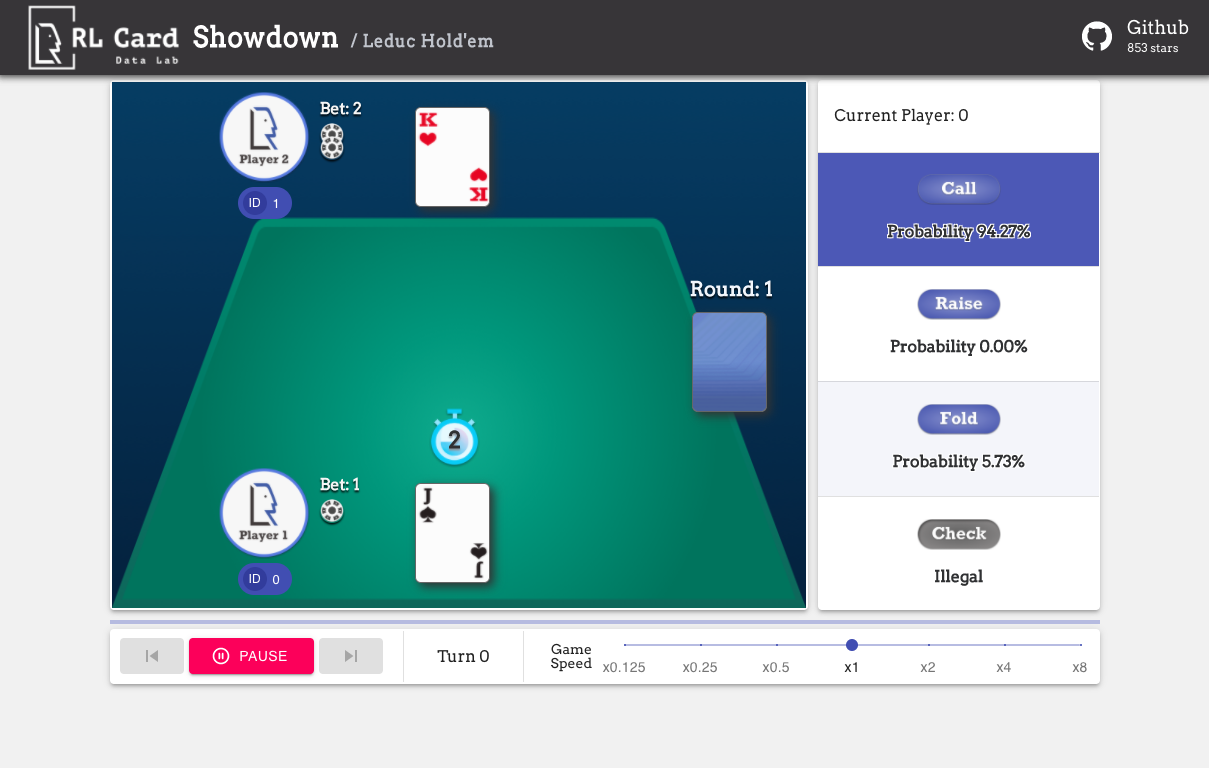
\includegraphics[height=.3\textheight]{rlcard-showdown}
                  \caption{RL Card Showdonw}
        \end{figure}
    \end{itemize}
\end{frame}

%%%

\begin{frame}
    \frametitle{Implementation}
    \begin{itemize}
        \item Structure for implemented games
        \begin{itemize}
            \item Game: contains players, dealer, round, payoffs
            \item Round: process of a round in a game
            \item Dealer: shuffling and giving cards
            \item Player: plays the cards following a strategy
            \item Judger: decides winner
        \end{itemize}
        \item Train different models to the implemented game
    \end{itemize}
\end{frame}

%%%

\begin{frame}
    \frametitle{Important Methods}
    \begin{itemize}
        \item perform\textunderscore draw\textunderscore action: handling when player draws a card
        \item perform\textunderscore card\textunderscore action: handling when player plays a card
        \item get\textunderscore legal\textunderscore actions: allowed cards in the given situation
        \item Reward function get\textunderscore payoffs: Decides how many points the winner/penalty points the loser gets
        \item RL algorithm tries to optimize the reward function
    \end{itemize}
\end{frame}
